\documentclass[12pt]{report}
\usepackage[a4paper]{geometry}
\usepackage[myheadings]{fullpage}
\usepackage{fancyhdr}
\usepackage{lastpage}
\usepackage{graphicx, wrapfig, subcaption, setspace, booktabs}
\usepackage{fourier}
\usepackage[protrusion=true, expansion=true]{microtype}
\usepackage[english]{babel}
\usepackage{sectsty}
\usepackage{url, lipsum}
\usepackage{tgbonum}
\usepackage{hyperref}
\usepackage[table]{xcolor}
\usepackage{listings}
\usepackage{color}
\usepackage[default]{lato}
\usepackage[T1]{fontenc}
\usepackage{titlesec}
\usepackage{multirow}
\usepackage{listings}

\definecolor{codegreen}{rgb}{0,0.6,0}
\definecolor{codegray}{rgb}{0.5,0.5,0.5}
\definecolor{codepurple}{rgb}{0.58,0,0.82}
\definecolor{backcolour}{rgb}{0.95,0.95,0.92}
\definecolor{dkgreen}{rgb}{0,.6,0}
\definecolor{dkblue}{rgb}{0,0,.6}
\definecolor{dkyellow}{cmyk}{0,0,.8,.3}
\definecolor{mygray}{rgb}{0.5,0.5,0.5}


\lstset {
	breaklines=true,
	upquote=true
}

\lstdefinestyle{PHP}{
	language = php,
	backgroundcolor=\color{backcolour},
	basicstyle = \small\ttfamily,
	numbers=left,
	numbersep=5pt,
	numberstyle=\tiny\color{mygray},
	tabsize = 2,
	upquote=true,
	keywordstyle = \color{dkblue},
	stringstyle = \color{red},
	identifierstyle = \color{dkgreen},
	commentstyle = \color{gray},
	emph = [1]{php},
	emphstyle = [1]\color{black},
	emph = [2]{if,and,or,else},
	emphstyle = [2]\color{dkyellow},
	showspaces=false,
	showstringspaces=false
}

\onehalfspacing
\setcounter{tocdepth}{5}
\setcounter{secnumdepth}{5}

% set chapter format
\titleformat{\chapter}[block]
{\normalfont\huge\lato}{\thechapter}{1em}{\Huge}
\titlespacing*{\chapter}{0pt}{-19pt}{0pt}

% remove red boxes
\hypersetup{%
	pdfborder = {0 0 0}
}

% change the link style you can use
\newcommand{\link}[1]{{\color{blue}\href{#1}{#1}}}

%-------------------------------------------------------------------------------
% HEADER & FOOTER
%-------------------------------------------------------------------------------
\pagestyle{fancy}
\setlength\headheight{15pt}
\fancyhead[L]{Wreath Network Penetration Test}
\fancyhead[R]{Chocolate Overflow}

%-------------------------------------------------------------------------------
% TITLE PAGE
%-------------------------------------------------------------------------------
\title{Wreath Network Penetration Test}
\author{Chocolate Overflow}

\makeatletter
\renewcommand{\maketitle}{
	\begin{titlepage}
		\begin{center}
			\large
			\vspace*{1cm}
			{\LARGE\@title}
			\par\vspace{1ex}
			\begin{tabular}[t]{c}
				by \@author
			\end{tabular}
			\vfill
			\par\vspace{1ex}
      Start of testing: August 10, 2021\\
			End of testing: August 11, 2021\\
		\end{center}
		\@thanks
	\end{titlepage}
}
\makeatother

\begin{document}
		\maketitle

		% nessuna numerazione
		\pagenumbering{gobble}
		\tableofcontents
		\newpage

		%-------------------------------------------------------------------------------
		% BODY
		%-------------------------------------------------------------------------------
		\pagenumbering{arabic}
		\chapter{Executive Summary}

In this penetration test, Mr. Thomas Wreath's network was examined for security weaknesses. This test was a grey-box test, with a rough layout of the network described. The scope of the assessment was as follows:
\begin{itemize}
	\item Public Facing Web Server: 10.200.177.200
	\item 2 other machines on the 10.200.177.0/24 network:
	\begin{itemize}
    \item Git Server
    \item Personal Computer
	\end{itemize}
\end{itemize}

Table ~\ref{tbl:targets} contains the overview of examined systems during the penetration test.
\begin{table}[h]
	\centering
	\begin{tabular}{|l|l|}
		\hline
		\textbf{IP address} & \textbf{Hostnames}\\
		\hline
		10.200.177.200 & thomaswreath.thm, prod-serv\\
		\hline
		10.200.177.150 & git-serv\\
		\hline
		10.200.177.100 & wreath-pc\\
		\hline
	\end{tabular}
	\caption{Targets examined during the penetration test}
	\label{tbl:targets}
\end{table}

As a result of the test, several high severity vulnerabilities have been identified among the assets in scope, some of which are of significant risk. Vulnerabilities of highes risks include: Out-of-date Software, Web Services running as High-privilege Users, Weak Credentials, and Insecure Administrative Settings.

		\newpage

		\chapter{Vulnerability Overview}
Table \ref{tbl:vuln overview} depicts all vulnerabilities found during the penetration test. They are categorized by their risk and potential and are differentiated in the categories low (green), medium (yellow), high (orange) and critical (red).

\begin{table}[h]
	\begin{tabular}{| l | l | p{7cm} | l | l |}
		\hline
		CVSS Score & Asset & Vulnerability & Section & Page\\
		\hline
		\cellcolor{red}10 & prod-serv & CVE-2019-15107: Command Injection &  \ref{ss:issue-1} & \pageref{ss:issue-1} \\
		\hline
		\cellcolor{red}10 & git-serv & Unauthenticated Remote Code Execution & \ref{ss:issue-2} & \pageref{ss:issue-2} \\
		\hline
		\cellcolor{yellow}6.8 & wreath-pc & Arbitrary File Upload & \ref{ss:issue-3} & \pageref{ss:issue-3} \\
		\hline
		\cellcolor{orange}7.8 & wreath-pc & Unquoted Service Path & ~\ref{ss:issue-4} & ~\pageref{ss:issue-4} \\
		\hline
	\end{tabular}
	\caption{Vulnerability overview}
	\label{tbl:vuln overview}
\end{table}

		\newpage

		\chapter{Results}
In this chapter, the vulnerabilities found during the penetration test are presented. All the issues are grouped by target and contain the following information:
\begin{itemize}
	\item Brief description.
	\item CVSS Base Score -- see \href{https://www.first.org/cvss/user-guide}{\textcolor{blue}{\underline{here}}} for details.
	\item Exploitability -- describes the likelihood of an issue being used against customer's infrastructure.
	\item Business impact.
	\item References to classifications: WASC, OWASP, CWE.
	\item Steps to reproduce.
\end{itemize}

\newpage

\section{Public facing web server}
\textbf{Hostnames}: thomaswreath.thm, prod-serv\\
\textbf{Server IP address}: 10.200.177.200

This is the only public facing server among the targets. The page on ports 80 and 443, which reveal the hostname \lstinline{thomaswreath.thm}, are simply a static page with nothing exploitable. The web service on port 10000, however, is vulnerable to CVE-2019-15107 and is ran as root, thus giving me an easy exploitation to become root on the server.\\

\subsection{CVE-2019-15107: Command Injection} \label{ss:issue-1}
The version of Minserv (1.890) running on the server has a known vulnerability CVE-2019-15107, giving us code execution on the server. In addition, the server is running as root, thus giving us code execution as root.

Basic information about this issue is presented in Table \ref{tbl:issue-1}.
\begin{table}[h]
	\centering
	\begin{tabular}{| l | p{10cm} |}
		\hline
		Description & CVE-2019-15107: Command Injection as root \\
		\hline
		CVSS Base Score & 9.8 \\
		\hline
		Exploitablity & High \\
		\hline
		Business impact & Total control over server. \\
		\hline
    References to classifications & CWE-78, CWE-250 \\
		\hline
	\end{tabular}
\caption{Issue \#1: Command Injection as root}
\label{tbl:issue-1}
\end{table}

\subsubsection{Minimal proof of concept}
\begin{enumerate}
    \item Download PoC from https://github.com/MuirlandOracle/CVE-2019-15107
    \item run exploit: \lstinline{./CVE-2019-15107.py thomaswreath.thm}
\end{enumerate}

\subsubsection{Proposed solutions} \label{solution:issue-1}
Update Minserv

\newpage

\section{Git Server}
\textbf{Hostname}: git-serv\\
\textbf{Server IP address}: 10.200.177.150

This git server is internal and is said to contain code of Mr.Wreath's code for his website. The git server is running an old version of GitStack vulnerable to a well-known Unauthenticated Remote Code Execution exploit and is running the web service as "nt authority\textbackslash system".

\subsection{Unauthenticated Remote Code Execution} \label{ss:issue-2}
The version of GitStack running on the git server is vulnerable to Unauthenticated Remote Code Execution with a pre-made PoC. Additionally, the web server is running as "nt authority\textbackslash system", thus running the PoC immediately gives us code execution as "nt authority\textbackslash system" on git-serv.

Basic information about this issue is presented in Table \ref{tbl:issue-2}.
\begin{table}[h]
	\centering
	\begin{tabular}{| l | p{10cm} |}
		\hline
		Description & Unauthenticated Remote Code Execution as "nt-authority\textbackslash system" \\
		\hline
		CVSS Base Score & 10.0 \\
		\hline
		Exploitablity & High \\
		\hline
		Business impact & Complete control over server, source code leakage.  \\
		\hline
    References to classifications & CWE-78, CWE-250 \\
		\hline
	\end{tabular}
\caption{Issue \#2: Unauthenticated Remote Code Execution}
\label{tbl:issue-2}
\end{table}

\subsubsection{Minimal proof of concept}
\begin{enumerate}
  \item Download exploit: \href{https://www.exploit-db.com/exploits/43777}{https://www.exploit-db.com/exploits/43777}
  \item Modify explioit to change backdoor location (modified exploit in section \ref{appendix-1}, page \pageref{appendix-1})
  \item Run exploit
  \item Acquire and use backdoor at \lstinline{/web/exploit-chocola.php}
\end{enumerate}

\subsubsection{Proposed solutions} \label{solution:issue-2}
Update GitStack

\newpage

\section{Personal PC}
\textbf{Hostname}: wreath-pc\\
\textbf{Server IP address}: 10.200.177.100
The web service running on port 80 uses the source code found in git-serv. Analyzing the source code, we're able to identified a flawed filter in the file upload functionality and abuse it to upload PHP code, giving us code execution. With a shell on wreath-pc, we find that the service "SystemExplorerHelpService" is vulnerable to "SystemExplorerHelpService", which we use to become "nt authority\textbackslash system" on wreath-pc.

\subsection{Arbitrary File Upload} \label{ss:issue-3}
The file upload filter checks the 2nd instead of the last extension in the file name of the uploaded file, making it possible to run PHP code by uploading a file whose 2nd extension is that of an image and last extension is ".php".

Basic information about this issue is presented in Table \ref{tbl:issue-3}.
\begin{table}[h]
	\centering
	\begin{tabular}{| l | p{10cm} |}
		\hline
		Description & Insufficient validation of uploaded files allow for upload of PHP files, leading to execution of arbitrary PHP code on the server \\
		\hline
		CVSS Base Score & 6.8 \\
		\hline
		Exploitablity & Medium \\
		\hline
		Business impact & Total compromise of source code, no immediate impact on availability.  \\
		\hline
		References to classifications & CWE-434, CWE-646 \\
		\hline
	\end{tabular}
	\caption{Issue \#3: Improper Validation of Uploaded Files}
	\label{tbl:issue-3}
\end{table}

\subsubsection{Minimal proof of concept}
\begin{enumerate}
  \item Create a valid image file (e.g. PNG)
  \item Create a one-line PHP code to be executed
  \item Embed PHP code in image: \lstinline{exiftool -Comment=<PHP one-liner> filename.png.php}
  \item Upload malicious image file
  \item Goto \lstinline{/resources/uploads/filename.png.php} to execute PHP code
\end{enumerate}

\subsubsection{Proposed solutions} \label{solution:issue-3}
Implement stricter file validation, checking the last file extension instead of the 2nd.

\subsection{Unquoted Service Path} \label{ss:issue-4}
Ther service "SystemExplorerHelpService" has its path unquoted and with spaces. Additionally, a directory in the unquoted path is given "FullControl" access the our user, which is excessive privilege. Together, they make it possible to trick Windows into running a malicious file elsewher in the path

Basic information about this issue is presented in Table \ref{tbl:issue-4}.
\begin{table}[h]
	\centering
	\begin{tabular}{| l | p{10cm} |}
		\hline
		Description & Unquoted Path of the Service "SystemExplorerHelpService" allows escalation to the user "nt-authority\textbackslash system" \\
		\hline
		CVSS Base Score & 7.8 \\
		\hline
		Exploitablity & High \\
		\hline
		Business impact & Total control over machine \\
		\hline
		References to classifications & CWE-428 \\
		\hline
	\end{tabular}
	\caption{Issue \#4: Unquoted Service Path}
	\label{tbl:issue-4}
\end{table}

\subsubsection{Minimal proof of concept}
\begin{enumerate}
  \item Write program to execute desired code (code used is in section \ref{appendix-2}, page \pageref{appendix-2})
  \item Place compiled binary in "C:\textbackslash Program Files (x86)\textbackslash System Explorer\textbackslash System.exe"
  \item Restart the service "SystemExplorerHelpService" (stop/start or wait until machine is restarted)
\end{enumerate}

\subsubsection{Proposed solutions} \label{solution:issue-4}
Change the service to use the fully quoted path.

		\newpage

		\chapter{Attack Narrative}
In this chapter, we go through the process of exploiting the Wreath network, providing reproduceable steps of the entire exploitation process. Table ~\ref{tbl:event timeline} lists all key events with their respective time stamps. All events took place on August 10th 2021.

\begin{table}[h]
  \centering
  \begin{tabular}{|l|p{15cm}|}
    \hline
    Time & Event \\
    \hline
    13:00 & nmap scans on 10.200.177.200 \\
    \hline
    13:10 & exploit CVE-2019-15107 to get root on prod-serv \\
    \hline
    13:12 & Exilftrated root's id\_rsa and SSH as root \\
    \hline
    13:18 & Uploaded nmap to /tmp/nmap-chocola \\
    \hline
    13:18 & Ran nmap ping scan \\
    \hline
    13:18 & Ran nmap port scan on 10.200.177.150 and 10.200.177.100 \\
    \hline
    13:26 & Ran exploit 43777 from EDB and got backdoor \\
    \hline
    13:27 & Open port 17171 on prod-serv and got shell on git-serv \\
    \hline
    13:30 & Created administrative account "chocola" on git-serv \\
    \hline
    13:34 & RDP into git-serv as "chocola" and dumped password hashes with mimikatz \\
    \hline
    13:40 & Run Invoke-Portscan on wreath-pc from git-serv \\
    \hline
    13:42 & Uploaded chisel to git-serv \\
    \hline
    13:47 & Opened firewall on git-serv port 17171 TCP inbound \\
    \hline
    13:48 & Got forward proxy to 10.200.177.100 \\
    \hline
    13:52 & Went to "/resources" and uploaded malicious image file to get code execution \\
    \hline
    14:02 & Got reverse shell on 10.200.177.100 \\
    \hline
    14:04 & Uploaded and ran winPEAS on wreath-pc \\
    \hline
    14:16 & Uploaded System.exe, restart SystemExplorerHelpService, and got shell as "nt authority\textbackslash system" \\
    \hline
    14:20 & Dumped and exfiltrated SAM hashes \\
    \hline
  \end{tabular}
\caption{Event Timeline}
\label{tbl:event timeline}
\end{table}

\newpage

Going to "http://10.200.177.200", we're redirected to "thomaswreath.thm".

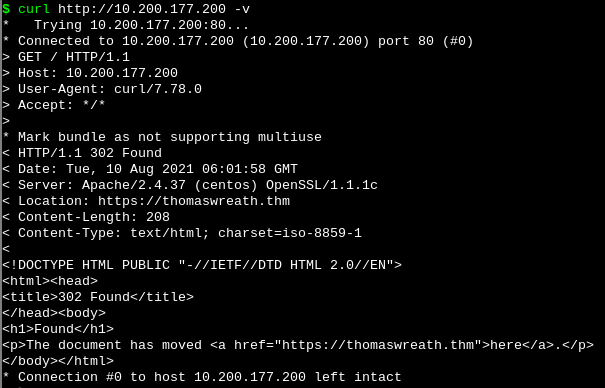
\includegraphics[width=\textwidth]{img/home-redirect.png}

Visiting the page, we only have a static page with nothing exploitable.

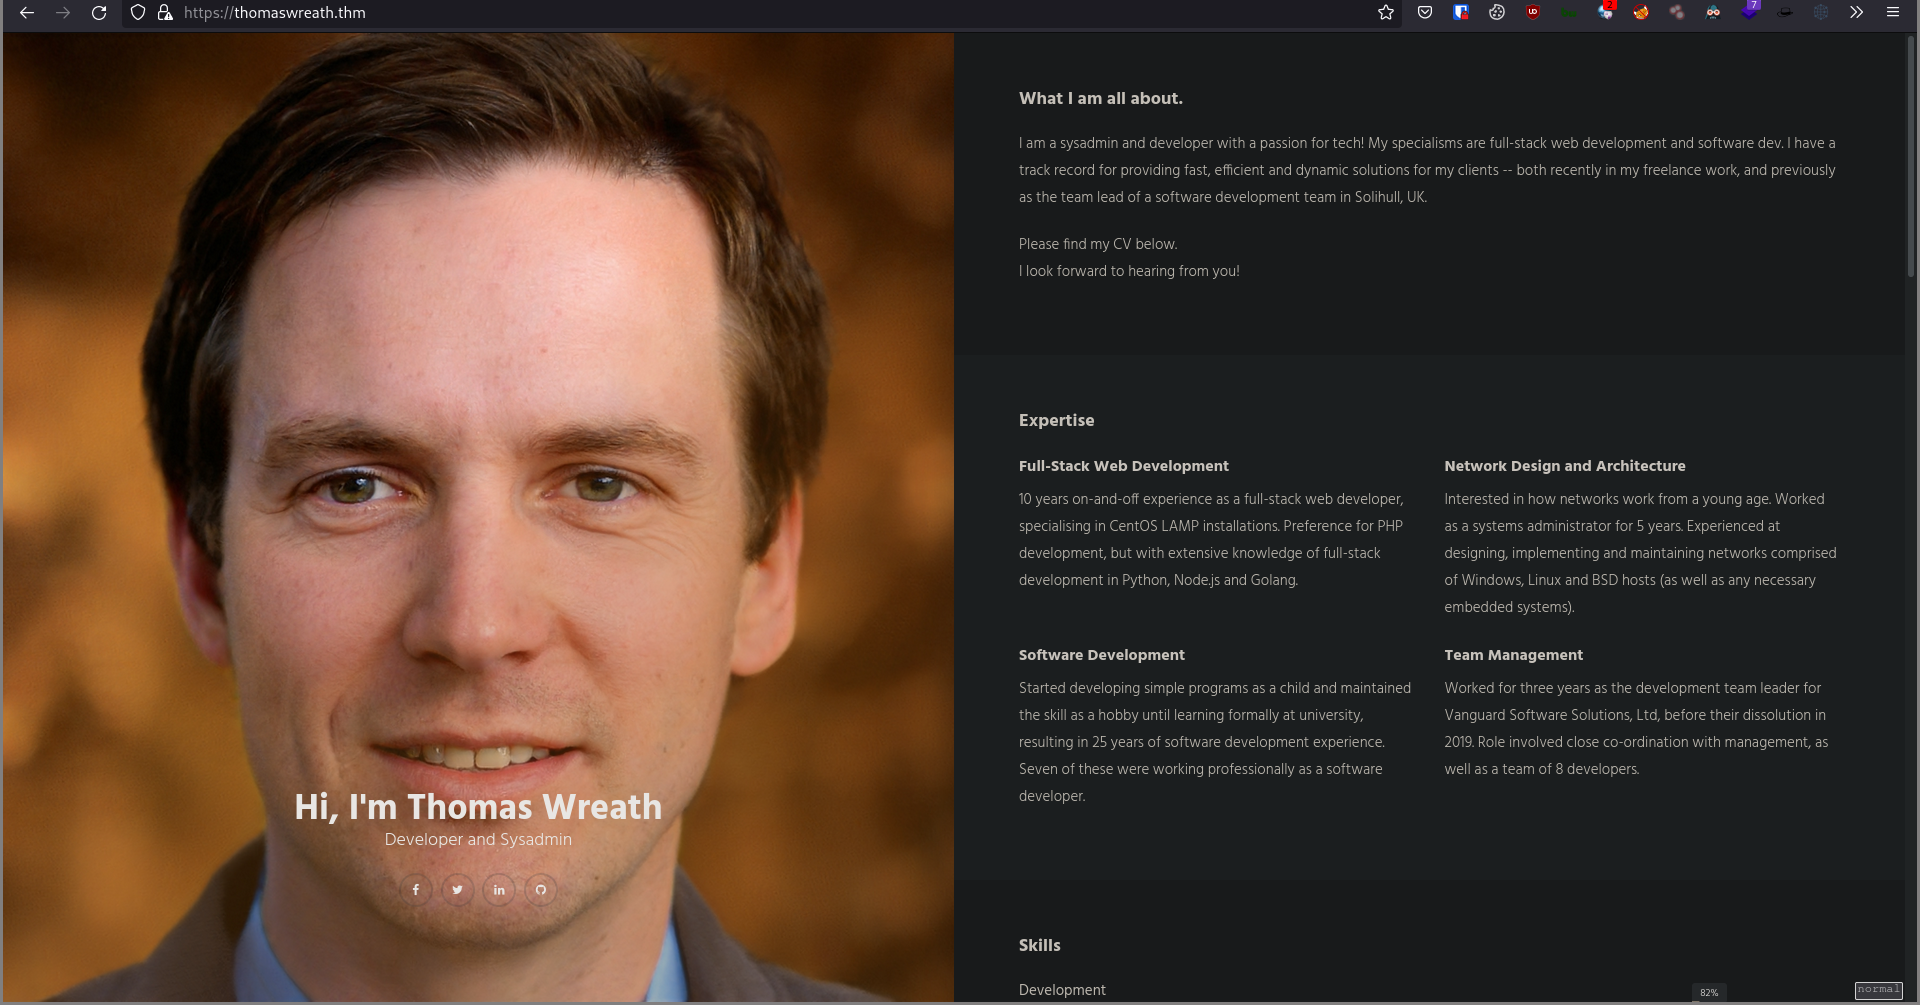
\includegraphics[width=\textwidth]{img/home.png}

The page on port 10000, however, is running an old version of Minserv (1.890) vulnerable to CVE-2019-15107, a Command Injection vulnerability, and has its web server running as root. Therefore, using an pre-made exploit, we can easily gain root access on the server.

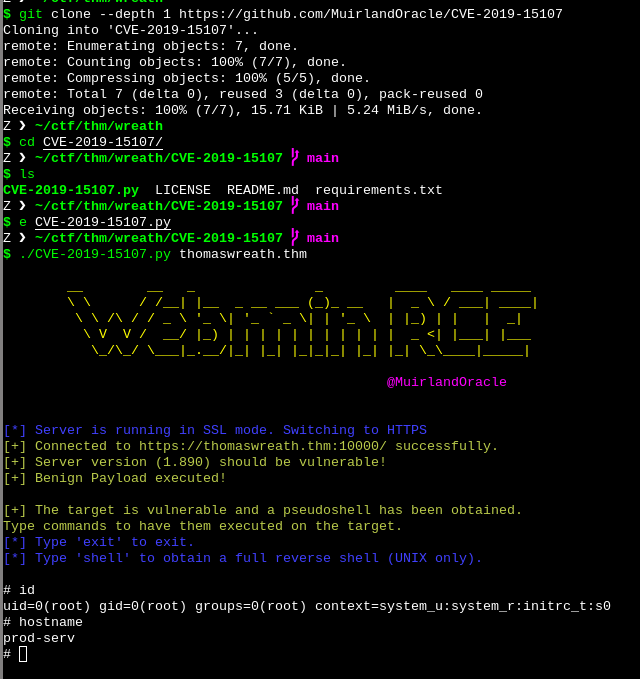
\includegraphics[width=\textwidth]{img/CVE-2019-15107.png}

With root access, I was able to exfiltrate and use root's existing id\_rsa file to impersonate and maintain access as root on prod-serv. After getting a binary of \lstinline{nmap} onto prod-serv, I did an IP scan and found 3 more IP addresses, of which only 10.200.177.100 and 10.200.177.150 are in scope.

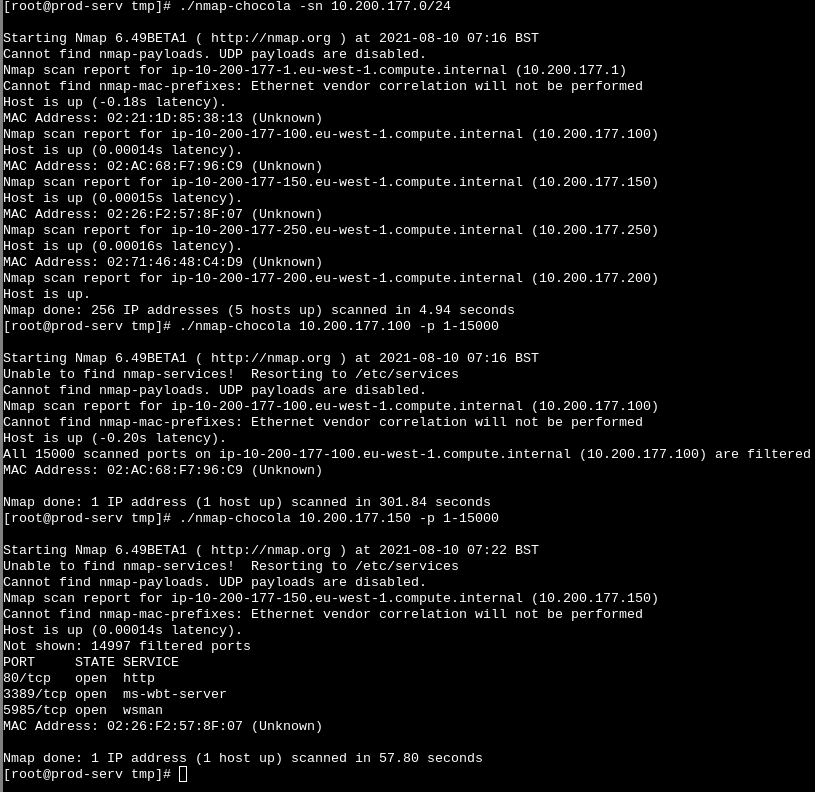
\includegraphics[width=\textwidth]{img/nmap-200.png}

As only 10.200.177.150 has open ports, I went on to enumerate it.

To get access to the internal servers, I ran \lstinline{sshuttle} with the previously found root id\_rsa on prod-serv.

\begin{lstlisting}[basicstyle=\footnotesize]
sshuttle -r root@thomaswreath.thm --ssh-cmd "ssh -i root.prod-serv.ssh" 10.200.177.0/24 -x 10.200.177.200
\end{lstlisting}

With the proxy set up, we're able to go to the web service running on git-serv.

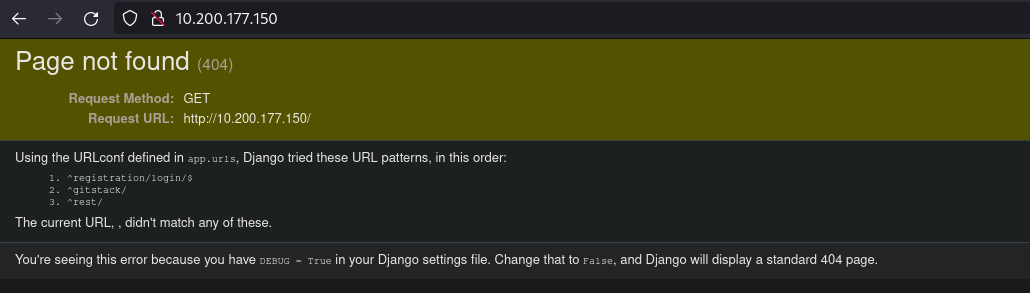
\includegraphics[width=\textwidth]{img/150-home.png}

We can see from the error message that there's a \lstinline{/gitstack} page. Looking for gitstack exploits, we can find exploit \href{https://www.exploit-db.com/exploits/43777}{43777} on Expoit Database. Running this exploit gives us a backdoor, and since the web service is running as "nt authority\textbackslash system", we have access to git-serv as said user.

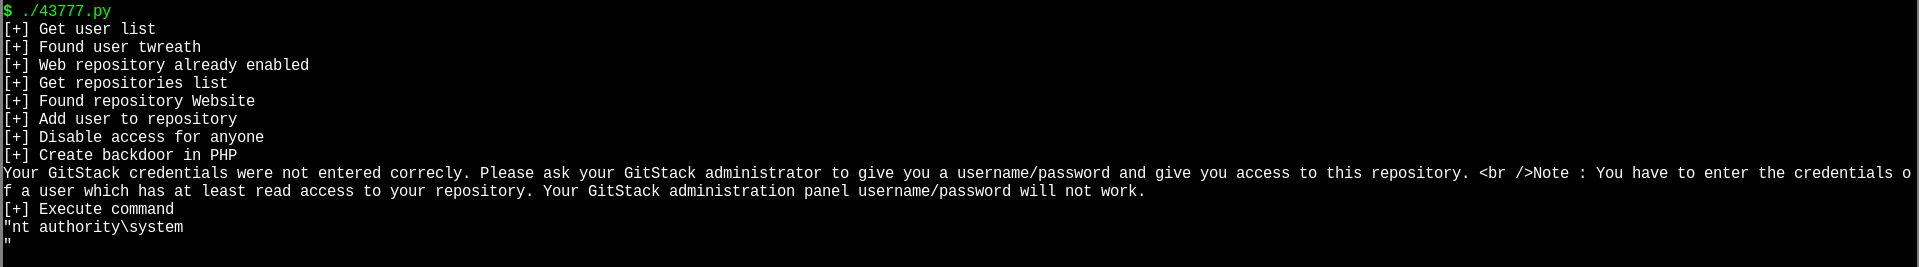
\includegraphics[width=\textwidth]{img/exploit-43777.py.png}

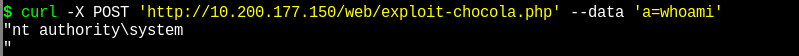
\includegraphics[width=\textwidth]{img/backdoor-43777.py.png}

Because traffic through unused ports are block on prod-serv, I opened port 17171 in the prod-serv's firewall to get a reverse shell on git-serv.

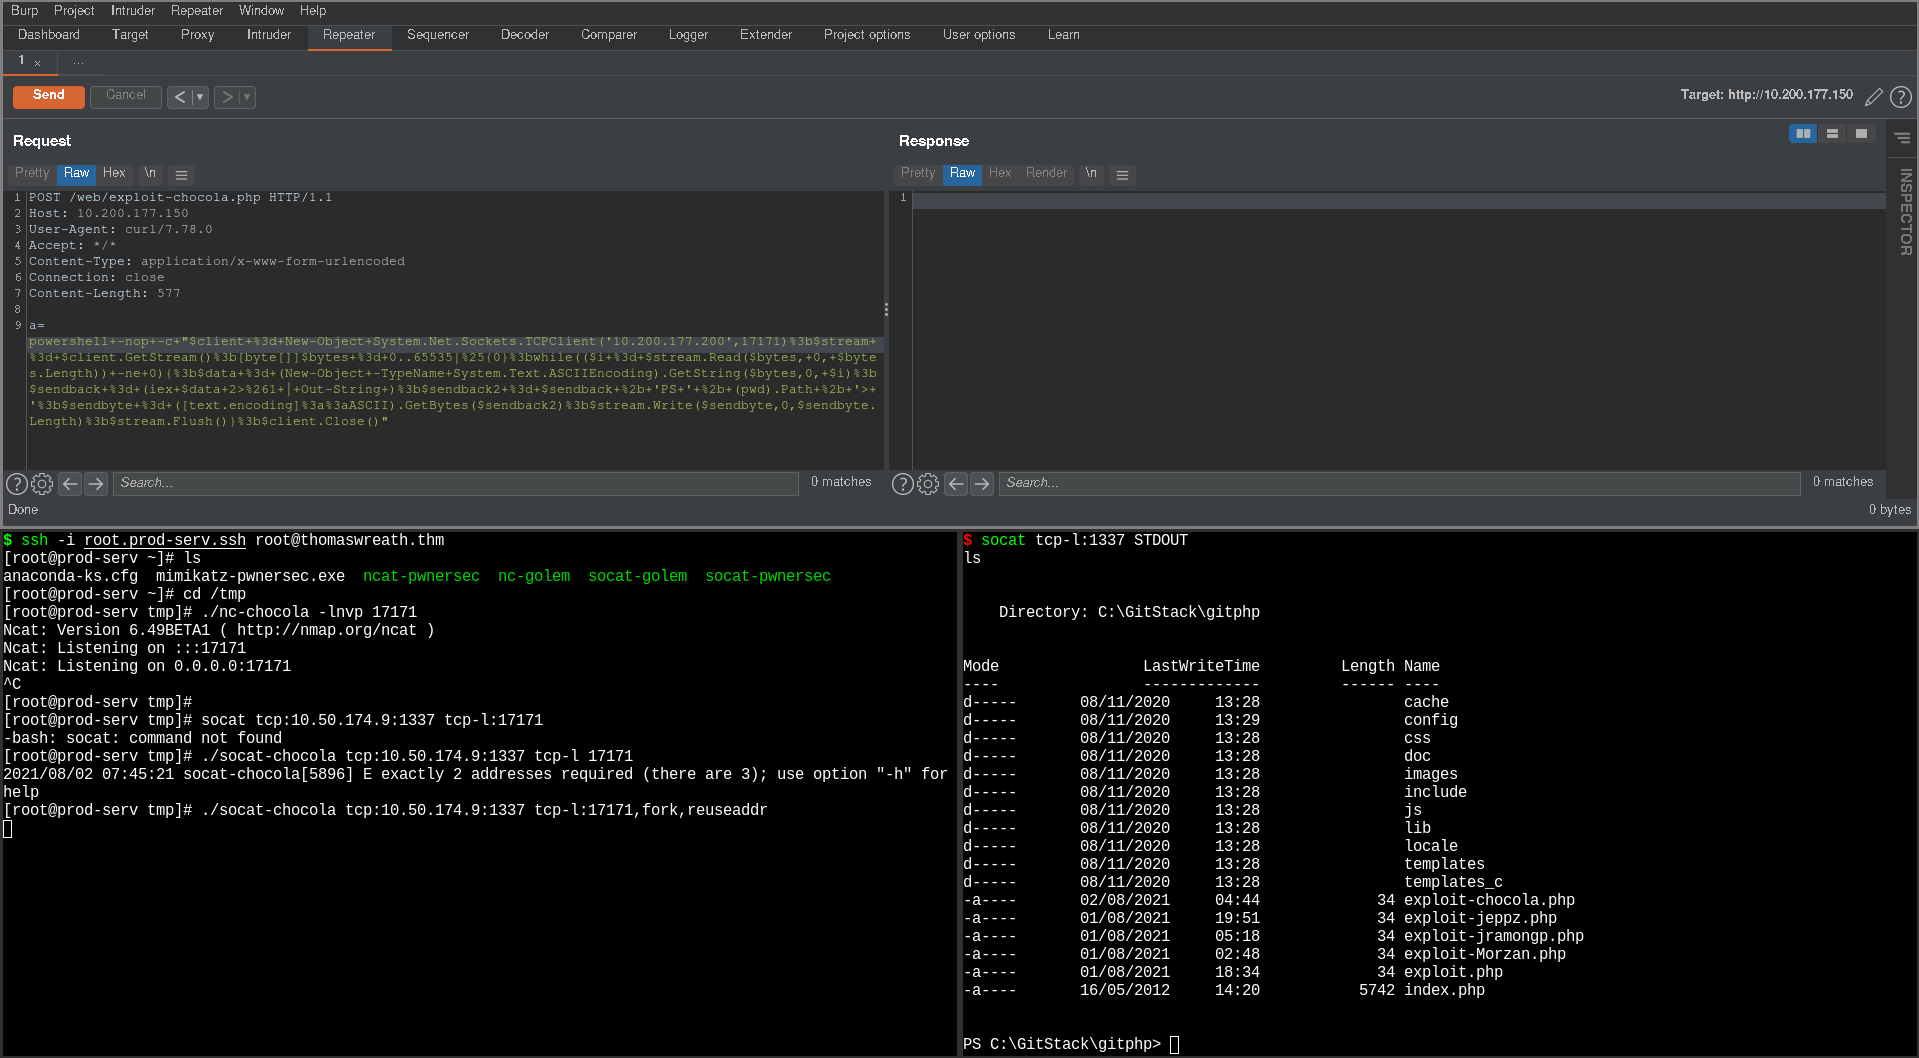
\includegraphics[width=\textwidth]{img/150-revshell.png}

With a shell, I created an Administrative account for persistence, as well as further leverage.

\begin{lstlisting}[basicstyle=\footnotesize]
net user chocola PASSWORD /add
net localgroup Administrators chocola /add
net localgroup "Remote Management Users" chocola /add
\end{lstlisting}

With the backdoor account, I logged in to git-serv through RDP and ran \lstinline{mimikatz} to dump password hashes.

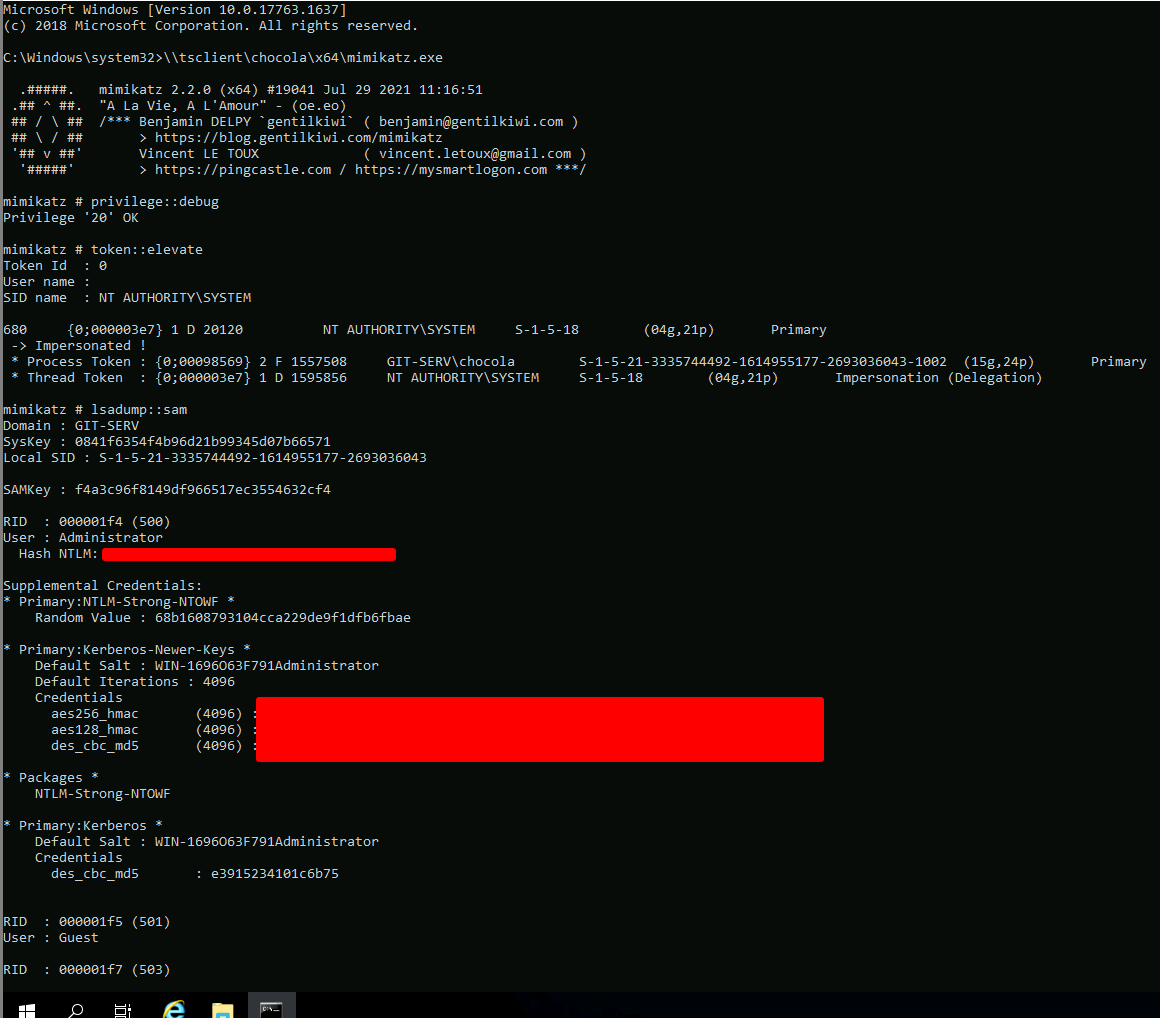
\includegraphics[width=\textwidth]{img/mimikatz.png}

Of the password hashes dumped, only Thomas' password could be cracked. However, I was also able to perform Pass-the-hash with Administrator's hash and get a shell with \lstinline{evil-winrm} as Administrator on git-serv. With this, I found the source code for Mr.Wreath's website on git-serv in \lstinline{C:\textbackslash GitStack\textbackslash repositories\textbackslash website.git}, which we'll come back to later in the report.

Using \href{https://github.com/EmpireProject/Empire/blob/master/data/module_source/situational_awareness/network/Invoke-Portscan.ps1}{Powershell-Empire's Invoke-Portscan} module, I scanned the last remaining machine on 10.200.177.100, and 2 ports were found: 80 and 3389.

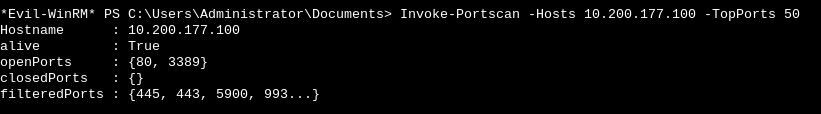
\includegraphics[width=\textwidth]{img/Invoke-Portscan.png}

Looking at the repository found in git-serv, The PHP code in \lstinline{/resources/index.php} is of interest to us.

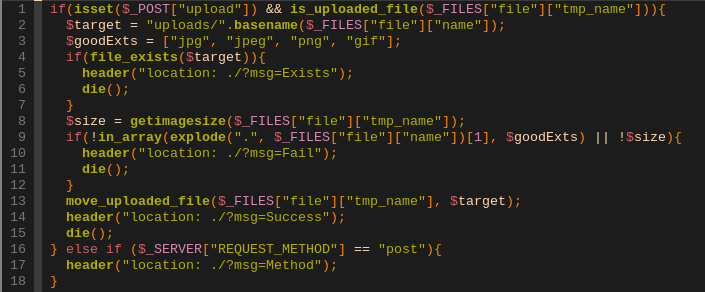
\includegraphics[width=\textwidth]{img/vuln-code.png}

There are 2 filters in place: a file extension whitelist and a image file type check. Regarding the 1st filter, in line 9 of the code above, the file name is split on "." and the 2nd item is checked against  a list of good extensions. This filter can easily be bypassed by having an extra extension in t he file name, for example "file.jpg.php" would pass the filter but still be a PHP file. As for the 2nd filter, it can be passed by uploading a legitimate image file with PHP code somewhere in the file.

To exploit the above vulnerability, a legitimate image file is created that a PHP code execution snippet is inserted as EXIF data, and the malicious image file is then uploaded to the server. This exploit will be used later in the engagement.

In order to reach 10.200.177.100, a hole was opened in git-serv's firewall (port 17171, TCP, inbound) and a binary of chisel was uploaded to git-serv in order to get a proxy. The proxy was acquired as follows:

\begin{lstlisting}
# 10.200.177.150
netsh advfirewall firewall add rule name="chisel-chocola" dir=in action=allow protocol=tcp localport=17171
./chisel-chocola.exe server -p 17171 --socks5

# attacker
chisel client git-serv:17171 9090:socks
\end{lstlisting}

With a proxy, I was able to reach the web server on 10.200.177.100. Going to \lstinline{/resources}, we're met with a Basic auth prompt, for which we can use Thomas' previously cracked credentials. With the previously analyzed file upload vulnerability, I uploaded a malicious image file to the server and got remote code execution.

With the payload on the server, I was able to upload a netcat binary (nc-chocola) to the machine (C:\textbackslash Windows\textbackslash temp\textbackslash nc-chocola.exe) and get a shell as "thomas" on wreath-pc.

With a shell, I then ran \href{https://github.com/carlospolop/PEASS-ng/blob/master/winPEAS/winPEASexe/binaries/Obfuscated\%20Releases/winPEASx64.exe}{winPEAS}. As a result, the service "SystemExplorerHelpService", which was running as Administrator, was found to have an unqoted path.

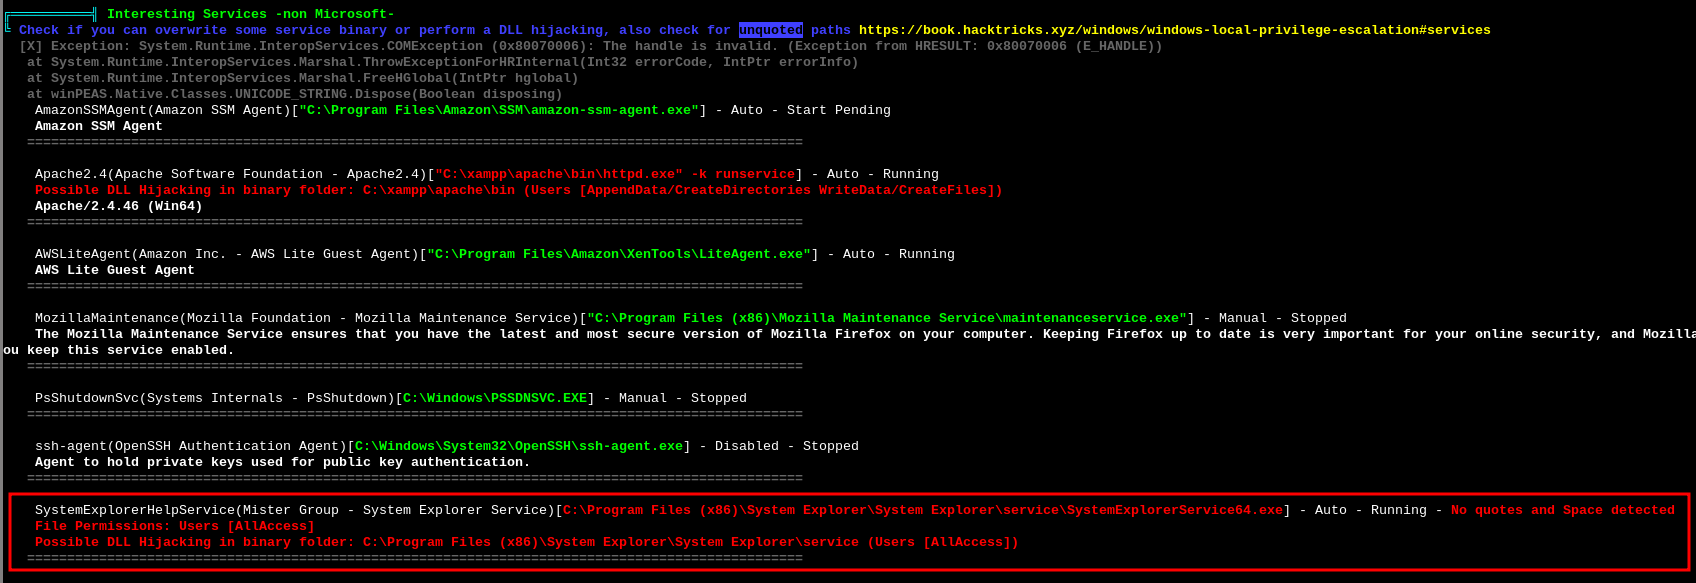
\includegraphics[width=\textwidth]{img/winpeas.png}

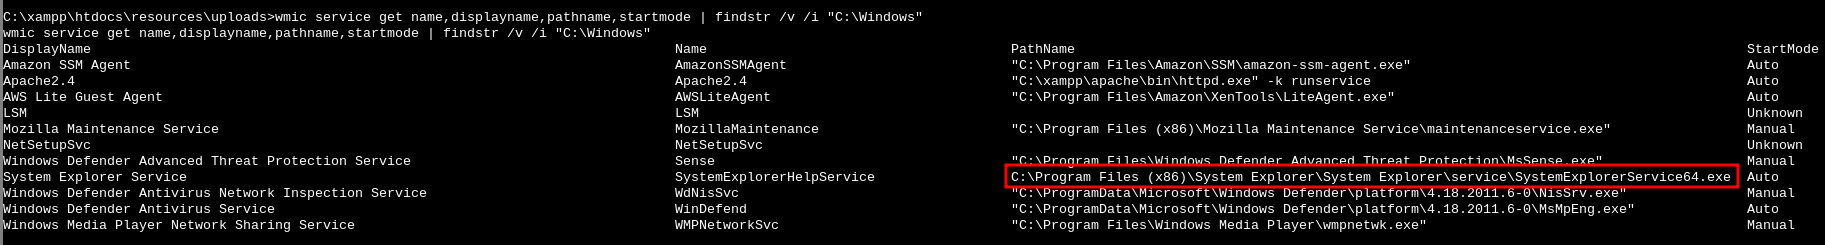
\includegraphics[width=\textwidth]{img/unquoted_service.png}

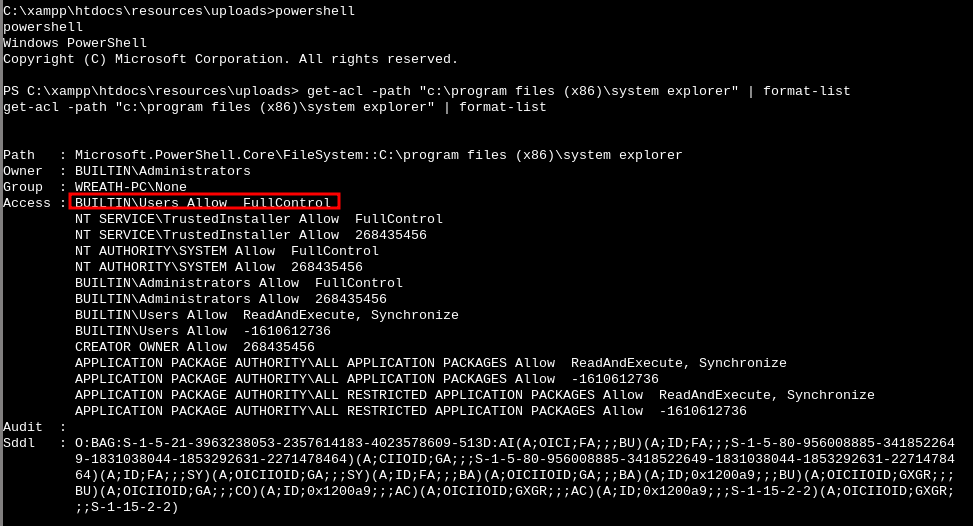
\includegraphics[width=\textwidth]{img/dir_fullcontrol.png}

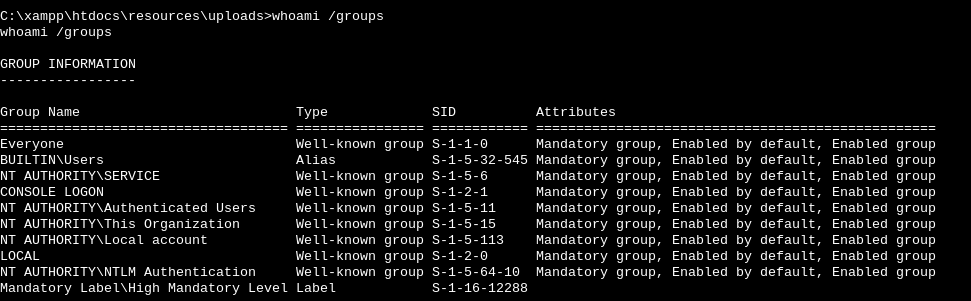
\includegraphics[width=\textwidth]{img/groups.png}

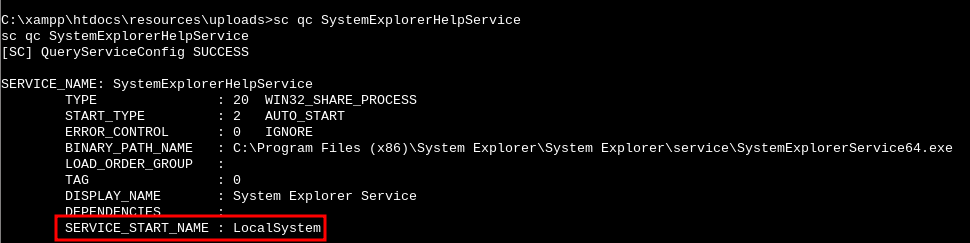
\includegraphics[width=\textwidth]{img/service_as_admin.png}

Additionally, an exploitable path, "C:\textbackslash Program Files (x86)\textbackslash System Explorer\textbackslash System Explorer", was found to have FullControl access by our user, specifically the group "BUILTIN\textbackslash Users". To exploit this, I compiled a wrapper program, whose code is in Appendix 2 (section \ref{appendix-2}, page \pageref{appendix-2}), and placed in on the machine as "C:\textbackslash Program Files (x86)\textbackslash System Explorer\textbackslash System.exe". With this, I was able to exploit the "Unquoted Service Path" vulnerability and get a shell as "nt authority\textbackslash system" on wreath-pc.

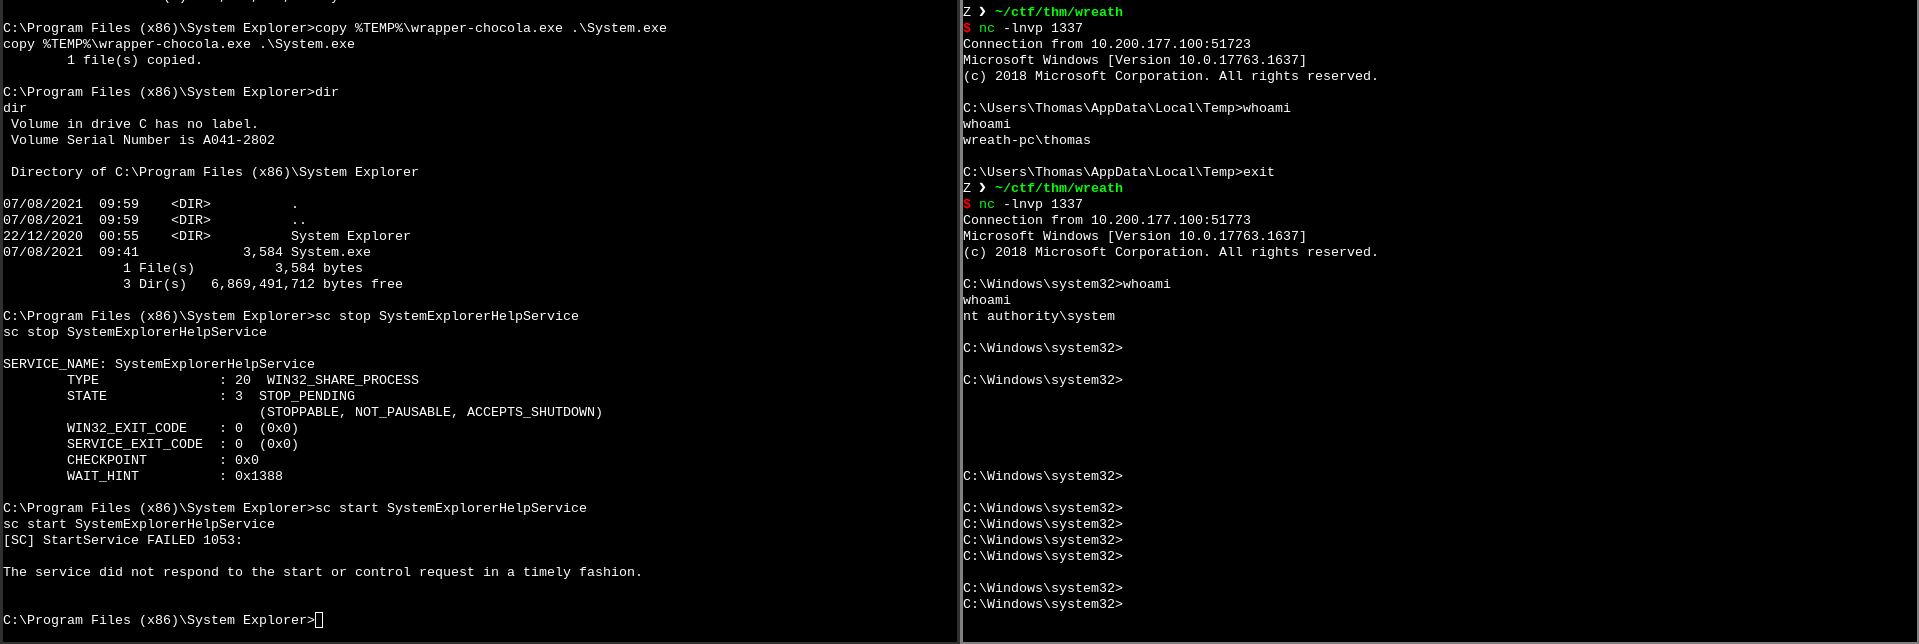
\includegraphics[width=\textwidth]{img/pc-system-shell.png}

With a shell as "nt authority\textbackslash system", I then exfiltrated and dumped password hashes as evidence.

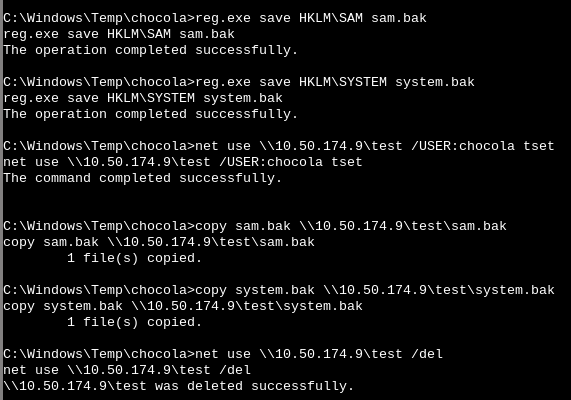
\includegraphics[width=\textwidth]{img/sam_dump.png}

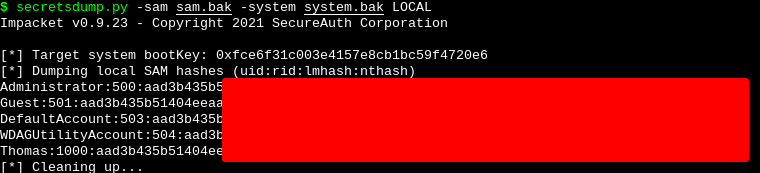
\includegraphics[width=\textwidth]{img/secretsdump.png}

		\newpage

		\chapter{Clean up}

This chapter lists all clean up actions done by the penetration tester. Cleanups are grouped by assets.

\section{10.200.177.200}

\begin{itemize}
  \item Delete files
    \begin{itemize}
        \item /tmp/nmap-chocola
        \item /tmp/socat-chocola
        \item /tmp/nc-chocola
    \end{itemize}
  \item Revert firewall (port 17171 TCP)
\end{itemize}

\section{10.200.177.150}

\begin{itemize}
  \item Revert firewall (port 17171 TCP)
\end{itemize}

\section{10.200.177.100}

\begin{itemize}
  \item Delete files
    \begin{itemize}
        \item C:\textbackslash windows\textbackslash temp\textbackslash nc-chocola.exe
        \item C:\textbackslash Program Files (x86)\textbackslash System Explorer\textbackslash System.exe
    \end{itemize}
\end{itemize}

		\newpage

		\chapter{Appendices}

\section{Appendix \#1: 43777.py} \label{appendix-1}
\lstinputlisting[basicstyle=\footnotesize,language=Python]{43777.py}

\newpage

\section{Appendix \#2: Wrapper.cs} \label{appendix-2}
\lstinputlisting[basicstyle=\footnotesize]{Wrapper.cs}

\end{document}
